\documentclass[12pt, a4paper, openright]{book}


\usepackage{amsmath}
\usepackage{graphicx}
\usepackage{hyperref}  % for citing URLs
\usepackage{listings}
\usepackage{float}
\lstset{breaklines=true}
\pagestyle{plain}
\newcommand{\HRule}{\rule{\linewidth}{0.5mm}}

\topmargin       0in
\oddsidemargin   0in
\evensidemargin  0in
\headheight      0in
\headsep         0in
\topskip         0in
\textheight      9in
\textwidth       6.5in

\begin{document}

\frontmatter
\begin{titlepage}
\begin{center}
\begin{spacing}{1.0}

% Upper part of the page. The '~' is needed because \\
% only works if a paragraph has started.

% Title
%\HRule \\[0.4cm]
~\\[0.3cm]
{ \LARGE \bfseries Experimental implementation of a cognitive radio using OpenBTS, GNU Radio and spectrum sensing techniques\\[1.2cm] }

%\HRule \\[1.5cm]
\textbf{\large M. Tech. Dissertation}\\[1.2cm]

{Submitted in partial fulfilment of the requirements for the degree of\\[0.1cm]
Master of Technology\\[0.3cm]
by\\[0.3cm]}

{\LARGE Abrar Ahmad\\[0.1cm]}
{1100000\\[1.1cm]}
{Supervisor\\[0.1cm]}
{\LARGE Prof.~S~N~Merchant\\[1.3cm]}


\includegraphics[width=0.21\textheight]{iitbLogo}~\\[0.9cm]
Department of Electrical Engineering\\[0.2cm]
\textbf{\large IIT Bombay}\\[1.3cm]

%\textsc{\Large Master of Technology Project}\\[0.5cm]
%
%
%% Author and supervisor
%\begin{minipage}{0.4\textwidth}
%\begin{flushleft} \large
%\emph{Author:}\\
%Abrar \textsc{Ahmad}\end{flushleft}
%\end{minipage}
%\begin{minipage}{0.4\textwidth}
%\begin{flushright} \large
%\emph{Supervisor:} \\
%Prof.~S~N \textsc{Merchant}
%\end{flushright}
%\end{minipage}

\vfill

% Bottom of the page
{\large \today}

\end{spacing}
\end{center}
\end{titlepage}

\chapter*{\centering{Abstract}}
Wireless networks are currently regulated by fixed spectrum assignment policy
which results in inefficient utilization of the spectrum. In the last few
years there has been a drastic increase in the mobile services, which in turn
has increased the demand for limited radio spectrum. Hence there is a need to
change the conventional static spectrum assignment policy and make efficient
utilization of spectrum. Cognitive Radio (CR) emerged as a new paradigm to
address the spectrum underutilization problem.  CR enables opportunistic use
of the radio-frequency spectrum by allowing Secondary/Un-licensed users to
utilize licensed bands under the condition that they should not cause the
interference with the Primary/Licensed users. Secondary users utilize the
detected free bands and leave them when the corresponding primary radio
emerges.

A USRP based two frequency CR Test-Bed and a four frequency CR Test-Bed has been
developed using GNURadio and OpenBTS to demonstrate these properties of
cognitive radio. Primary and secondary users are made to coexist with no
effect on the primary radio. Energy detection spectrum sensing technique is
used to detect the free bands also known as the spectrum holes. We demonstrate
that secondary users utilize these spectrum holes and vacate them whenever
primary users want to use them.


\setcounter{tocdepth}{2}
\tableofcontents

\listoffigures
\setlength{\parindent}{0em}
\setlength{\parskip}{1em}
\setlength\arraycolsep{2pt}

\mainmatter
\chapter{Introduction}
\pagenumbering{arabic}
\thispagestyle{empty}
\section{Motivation}
Due to the rapid increase of mobile phones and other wireless communication 
devices, 
there is a need for efficient utilization of the available radio spectrum.
The Spectrum Policy Task Force, a group under the Federal Communications  
Commission (FCC) in the United States, published a report in 2002 saying 
\cite{repFCC}: 
\begin{quote}
``In many bands, spectrum access is a more significant problem than physical
scarcity of spectrum, in large part due to legacy command-and-control 
regulation that limits the ability of potential spectrum users to obtain such 
access.''
\end{quote}
If we scan the spectrum in metropolitan cities which are heavily used regions,
we find that some frequency bands are unoccupied most of the time\cite{staple04}. These 
are referred to as spectrum holes. A spectrum hole is a band of frequencies 
assigned to a primary user, but, at a particular time and specific geographic 
location, the band is not being utilized by that user\cite{kolodzy01}.

\begin{figure}
\centering
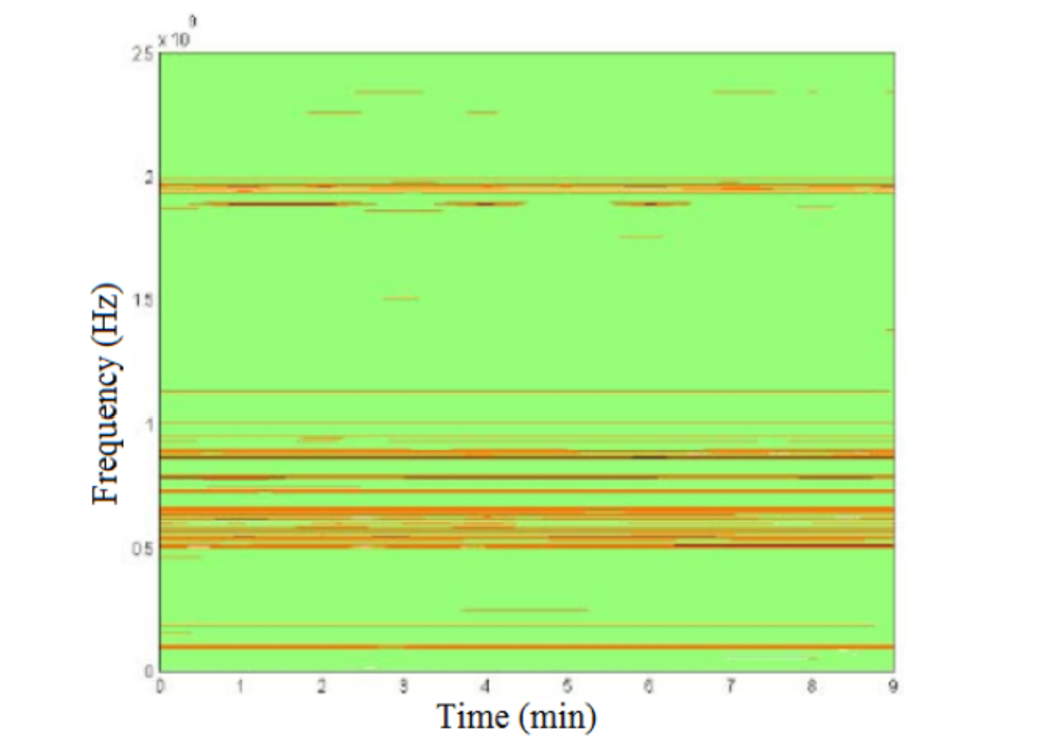
\includegraphics[width=0.7\textwidth]{../images/freqUsage}
\caption[Frequency usage of Spectrum Band]{Frequency usage of Spectrum Band {\cite{kranthi13}}}
\label{frequencyUsage}
\end{figure}


This problem of inefficient utilization of spectrum can be solved by allowing 
secondary users which are non licensed, to access these spectrum holes.
Cognitive radio which includes software defined radio, is a means to 
accomplish this by utilizing these spectrum holes intelligently and 
efficiently\cite{haykin05}\cite{mitola99}\cite{mitola00}. It uses one of the spectrum sensing techniques to 
identify the spectrum holes in the radio spectrum.


\section{Cognitive Radio}
A cognitive radio is an intelligent radio whose primary objective is efficient
utilization of the radio spectrum. It can be programmed and configured 
dynamically. It works on the principle of understanding-by-building to learn 
from the surrounding environment and adapt to changes in the RF stimuli by 
making corresponding changes in operating parameters. The transceiver is 
designed to find an unoccupied channel in the vicinity and utilize it for 
transmission. It enables coexistence of primary licensed users and secondary 
unlicensed users. Whenever a primary user wants to occupy the channel which is
currently in use by secondary users, it finds some other unoccupied channel in
the vicinity and secondary users migrate seamlessly to this new channel thus 
vacating the previously used channel for primary users.  

\section{Contribution of this Thesis}
An experimental setup is developed which demonstrates the presence of 
secondary users along with primary users in the existing GSM network and 
utilizing the already existing resources there by increasing the total 
mobiles in the network.
\begin{enumerate}
  \item A 2-frequency band cognitive system is developed where secondary 
  users migrate to frequency $f2$ if frequency $f1$ is occupied an viceverca.
  \item A 2-frequency system is extended to a 4-frequency system where 
  we demonstrate that primary users are occupying two bands out of these four
  and secondary users occupy one out of the other two free bands.
  \item We have used energy detection spectrum sensing technique and CUSUM
  peak detection technique to detect the presence of primary users. Band 
  occupied by secondary users is continuously monitored to check if primary 
  users are trying to occupy that band and as soon as the request from primary
  users is detected a new free band is found out in the vicinity and utilized 
  by secondary users for transmission there by vacating the band for primary 
  users . 
\end{enumerate}

\section{Organization of this Thesis}
The rest of this document is organized as follows. Chapter 2 briefly describes the GSM 
architecture and its Um interface. Chapter 3 discusses about software defined radio, GNURadio 
software and Universal Software Radio Peripheral (USRP N210), the hardware used in this 
project.OpenBTS software is described in Chapter 4. 
SIM registration and calling using local network  is described in chapter 5.
Chapter 6 covers spectrum sensing techniques to detect the presence of primary users in the 
channel.  Chapter 7 and 8 covers implementation of 2-Frequency and
4-Frequency cognitive radio test-beds using GNU Radio
and OpenBTS. Experimental setup for our project, 
detailed description of what we have achieved in this 
project along with the flow chart of our work is also covered in these chapters.
The final chapter of this thesis 
is the conclusion of our project followed by future work. 

\chapter{Spectrum Sensing}

Due to limited availability of spectrum resource, there is a serious impact on 
the emerging mobile applications. Hence there is a need to efficiently utilize
the available radio spectrum. The problem right now is not the physical scarcity
of the radio spectrum rather the inefficient use of the spectrum. Solution to 
this is cognitive radio. The major problems in cognitive radio is detection of 
primary users in the licensed spectrum and enable secondary users to quit the 
frequency band as quickly as possible if the corresponding primary radio emerges
to avoid interference to primary users. This technique is called spectrum 
sensing. Spectrum sensing is the first step to implement cognitive radio system.

There are various methods for local spectrum sensing proposed by researchers.

The following section describes three important methods:
\begin{enumerate}
	\item Energy detection
	\item matched filter detection 
	\item cyclo stationarity detection
\end{enumerate}

\section{Energy Detection}

Measuring the energy of a particular band is one of the simplest techniques to 
detect the presence of primary users in that band. It is one of the most widely
used technique to detect spectrum holes as it requires no a priori knowledge of 
the primary radio. Apart from this major advantage the technique is very cost 
efficient and less complex compared to other techniques. 
We calculate the energy of the received radio spectrum and this energy is 
compared with a predefined energy detection threshold to conclude whether 
primary user is present or absent in the frequency of interest. This technique 
is an optimal one when we have absolutely no knowledge of the user occupying the
channel in advance. The following block diagram describes energy detection 
technique:

Block diagram for energy detection technique from stage one report here:


As described in the energy detection block diagram, it is basically a hypothesis
testing problem with two possible hypothesis $H0$ and $H1$. Hypothesis $H1$ concludes 
the presence of primary users in the band of interest and hypothesis $H0$ 
concludes their absence. And energy detection technique is basically about 
distinguishing between these two hypothesizes.[3 from stage one report]

\begin{align}
x(t) & = n(t); & H0 \nonumber \\
x(t) & = hs(t)+n(t); & H1 \nonumber
\end{align}

where $x(t)$ is signal received by secondary user and $s(t)$ is primary radio 
signal, $n(t)$ is additive white Gaussian noise (AWGN) and $h$ is the amplitude gain
of the channel. $s(t)$ and $n(t)$ are assumed to be independent of each other. 
Signal detection is performed using an energy detector and compute decision 
statistics $Y$ which corresponds to energy collected in observation time $Y$ and 
bandwidth $W$ and comparing this statistics to a predetermined threshold. Energy 
detection is implemented using average periodogram analysis which is covered in 
later part of this report.


\section{Matched filter detection}
Matched filter is a linear filter used to match a particular transit waveform 
with the reference signal. The output is maximum when the match happens. When 
there is a priori knowledge of primary radio, matched filter technique is 
applied. Matched filter operation is equivalent to correlation operation in 
which the incoming signal is convolved with a filter whose impulse response is 
mirror and shifted version of reference signal. This output is then compared 
with the threshold for primary user detection. It is mathematically defined as:

\begin{equation*}
Y[n] = \sum_{k=-\infty}^{\infty}x[k]h[n-k]
\end{equation*}

$x$ is the unknown signal and $h$ is the impulse response of matched filter which is 
matched to reference signal for maximizing SNR. 

Block diagram of matched filter is given in fig:

There is a constraint on this technique. We need to have a prior information 
about the primary radio to perform matched filtering. However matched filter 
requires demodulation of primary signal which means it has information of 
primary radio both at the PHY layer and the MAC layer like operating frequency, 
modulation type, packet format bandwidth etc. But the cumbersome part is it has 
to achieve coherency with primary user by means of timing and carrier 
synchronization. This coherent detection is still achievable since primary 
signals have pilots, preambles etc to serve the purpose. 
The advantage of matched filter detection is when the information of the primary
user signal is known, it is optimal detection in stationary Gaussian noise. But 
the performance of matched filter detection depends on the accuracy of the 
information of primary radio. This technique also requires cognitive radio to 
have dedicated receiver for every type of primary user which in turn results in 
complex hardware and large power consumption. [4] kranti thesis

\section{Cyclostationarity detection}

This technique utilizes periodicity property of the received signal to detect 
presence of primary users. Periodicity property is generally exhibited by the 
communication signals due to sinusoidal carriers, pulse train, hopping sequences
etc. Due to this underlying periodicity most of the communication signals can be
modeled as cyclostationary processes[1from folder project on desktop]. This 
technique detects a random primary signal with a particular modulation type in a
background of noise and other modulated signals.

Cyclostationary feature detection is robust to noise and is a better performer 
than energy based detection in low SNR regions. This technique also requires a 
priori knowledge of the primary signal. Also this technique is computationally 
highly complex and the sensing time is also quiete long. Due the these reasons 
it is less commonly used than energy based detection.

Block diagram of cyclostationary detection is given in the figure:[14 from 
kranti thesis]


Diagram 

The detection is done by finding a unique cyclic frequency of the spectral 
correlation function of the received signal [4kranti]. The spectral correlation 
function is the Fourier transform of the cyclic autocorrelation function the 
spectral correlation function is defined as:
\begin{equation*}
        S(f,\alpha) = \int_{-\infty}^{\infty} R_{x}^{\alpha}(\tau)e^{-2 \pi f\tau}d\tau 
\end{equation*}

Where the cyclic autocorrelation function is defined by:
\begin{equation*}
    R_{x}^{\alpha} = E\{x(t+\tau)x^{*}(t-\tau)e^{-2 \pi \alpha t}\}
\end{equation*}

Here $x(t)$ is the signal received and $\alpha$ is the cyclic frequency. The spectral 
correlation function is also termed as cyclic spectrum.
This is a two dimensional transform unlike power spectral density which is 1 
dimensional. For successful detection under cyclo-stationary based spectrum 
sensing, we need a priori knowledge of the cyclo-stationary features of the 
received signal only. However matched filtering is the optimal solution when we 
completely know about received signal in advance.
This technique doesn't work well when the underlying noise is stationary. More 
over channel fading destroys the property of cyclo stationarty of the received 
signal and is also susceptible to sampling clock offset. 


Comparision of various spectrum detection techniques

Diagram from kranti's thesis 









The figure compares various spectrum sensing techniques on the basis of their 
accuracy and complexity. We can see that energy detection technique is the least
accurate and least complex of all where as matched filtering is most complex and
highly accurate. Other techniques lie in between with some having more accuracy 
and some less complex. There is no ideal detector that suits all occasions. Thus
decisions, compromises and tradeoffs must be made depending on primary radio 
type, transmission and propagation characteristics, characteristics of secondary
user receiver, and etc [2 from karanti thesis].

\section{Implementaton of energy detection technique}
We have used energy detection technique for spectrum sensing in our project for 
the detection of primary users in the band of interest. Average periodigram 
analysis is a method to implement energy detection technique of spectrum 
sensing. This section describes average periodogram analysis.  Implementation of
wide band spectrum analyzer using this technique is also described in this 
section.

\subsection{Average periodogram anaylsis}
Average Periodogram analysis estimates the power spectrum of the received signal
and it is based on the Discrete Fourier Transform (DFT) of finite length 
segments of signal. In this technique signal is sectioned into finite length 
segments and periodogram of each segment is calculated which are also referred 
to as modified periodograms. Then an average of all these modified periodogram 
is calculated.[8 from krantis report]

Let $X[n]; n = 0,1...L-1$ be the discrete time signal which is  divided into 
$M$ 
finite length segments of equal length, where $N$ is the length of each segment  
i.e. $ MN = L; X_{r}[n]; n = 0,1...N-1 $ is the $r$th segment and $ W[n]; n = 0,1...N-1 $ is 
the window applied to each segment. The modified periodogram for the $r$th segment
 is,
\begin{equation*}
    I_{r}[k] = \frac{1}{NU} \left| V_{r}[k]\right|^2     \qquad k = 0,1...N-1 
\end{equation*}
where $V_{r}[k]$ is a N point DFT and $U$ is normalization factor i.e. , 
$V_{r}[k] = DFT\{W[n]*X[n]\}$
and $U = \frac{1}{N}(\sum_{n-0}^{N-1} (W[n])^2)$
The PSD of $X[n]$ sequence is then the time averaged periodogram estimate ,
\begin{equation*}
    I[k] = \frac{1}{M}\left|\sum_{r=0}^{M-1}X_{r}[k]\right|
\end{equation*}

\section{Wide band spectrum analyzer}

GNU radio packages provide a tool for
wide band spectrum sensing 
called 
usrp\_spectrum\_sense.py. The program is provided in the appendix. 
It is used as
a basic code for wide band spectrum analyzer implementation. The output of this 
code is the magnitude squared of the FFT. This means for each FFT bin he output 
is $ Y[i] = re[X[i]]*re[X[i]] + im[X[i]]*im[X[i]]$. We can calculate the power by
taking square root of the output. We need $N$ time samples of $x(t)$ sampled at a 
sampling frequency of $F_{s}$ to use $N$ point complex FFT $X(\omega)$ analysis. An 
appropriate window function is to be selected to reduce spectral leakage and 
applied to these time samples. The output of the complex FFT will represent the 
frequency spectrum content as follows: The first value of the FFT output 
$(bin0 == X[0])$ is the passband centre frequency The first half of FFT spectrum 
($X[1]$ to $X[N/2-1]$) contains the positive baseband frequencies, which corresponds
to the passband spectrum from centre frequency to $+F_{s}/2$. The second half of the 
FFT ($X[N/2]$ to $X[N-1]$) contains the negative baseband frequencies, i.e. from 
$-F_{s}/2$ to centre frequency.


For our project purpose, we collected 1024 samples using a tuner centered at 
uplink frequency of our interest, say 900 MHz. 1024 is choosen as the number of 
FFT points because the number of FFT points has to be a power of 2 for the fast 
execution of the FFT algorithm. Default  sampling frequency is set as 10 MHz. 
The frequency resolution is therefore: 10 MHz / 1024 = 9.7656 MHz. The 
decimation is defined as dsp rate divided by sample rate. The UHD driver 
requires the decimation value to be an even number. The dsp rate is the actual 
hardware-level sampling rate of the USRP kit. It is the rate at which the USRP 
device takes analog samples from the external world and converts them to digital
form. The dsp rate of the USRP is 100 MHz. Hence we chose sampling frequency to 
be 10 MHz which gives a decimation value of: 100 MHz / 10 MHz = 10.


\appendix
%\chapter{Codes}

\section{Code for the two-frequency system}


\subsection{freq2secondaryBTS.py}

This code was written to demonstrate the two-frequency system.
This code was written by modifying the already available program named 
``usrp\_spectrum\_sense.py'' that comes together with the GNURadio software
package. We set the 
default UHD device address to ``192.168.20.2'' because that is the IP address
of the USRP device we are using as a spectrum sensor. The default samping rate
was set to 1e6 i.e. 1MHz. The default FFT size is given as 'sampling rate /
channel bandwidth'. We wanted an FFT size of 1024 so we set the bandwidth to
976.56 Hz since 1 MHz / 976.56 Hz $\approx$ 1024.

The class 'my\_top\_block' was modified by replacing the lines:
\begin{lstlisting}[language=Python]

        self.channel_bandwidth = options.channel_bandwidth

        self.min_freq = eng_notation.str_to_num(args[0])
        self.max_freq = eng_notation.str_to_num(args[1])

        if self.min_freq > self.max_freq:
            # swap them
            self.min_freq, self.max_freq = self.max_freq, self.min_freq    
\end{lstlisting}
with the lines
\begin{lstlisting}[language=Python]
        self.channel_bandwidth = options.channel_bandwidth

        self.down_freq = eng_notation.str_to_num(args[0])
        self.up_freq = (self.down_freq) - 45e6    
\end{lstlisting}

The method 'set\_next\_freq' of the class 'my\_top\_block' was modified by
replacing
\begin{lstlisting}[language=Python]
        target_freq = self.next_freq
        self.next_freq = self.next_freq + self.freq_step
        if self.next_freq >= self.max_center_freq:
            self.next_freq = self.min_center_freq
\end{lstlisting}
with
\begin{lstlisting}[language=Python]
        target_freq = self.up_freq
\end{lstlisting}




In the code listing that follows we have listed only the functions that we
customized and the ones that we added.

\begin{lstlisting}[language=Python]
def main_loop(tb):
    startOpenBTS(tb.down_freq,tb)

    
def sub_loop(tb):

    # use a counter to make sure power is less than threshold
    # lowPowerCount = 0
    # lowPowerCountMax = 10
    print 'fft size', tb.fft_size
    N = tb.fft_size
    mid = N // 2
    cusum = 0
    counter = 0
    

    while 1:

        # Get the next message sent from the C++ code (blocking call).
        # It contains the center frequency and the mag squared of the fft
        m = parse_msg(tb.msgq.delete_head())

        # m.center_freq is the center frequency at the time of capture
        # m.data are the mag_squared of the fft output
        # m.raw_data is a string that contains the binary floats.
        # You could write this as binary to a file.



        center_freq = m.center_freq
        bins = 102
        power_data = 0
        noise_floor_db = 0 ## 10*math.log10(min(m.data)/tb.usrp_rate)
        
        for i in range(1, bins+1):
            power_data += m.data[mid-i] + m.data[mid+i]
        power_data += m.data[mid]
        power_data /= ((2*bins) + 1)
        
        power_db = 10*math.log10(power_data/tb.usrp_rate) - noise_floor_db
        power_threshold = -59.0
        
        

        #if (power_db > tb.squelch_threshold) and (power_db > power_threshold):
            #print datetime.now(), "center_freq", center_freq, "power_db", power_db, "in use"
            # lowPowerCount = 0
        #else:
        print datetime.now(), "center_freq", center_freq, "power_db", power_db
            # lowPowerCount += 1

        # if (lowPowerCount > lowPowerCountMax):
        # down_freq = center_freq + 45e6
        # startOpenBTS(down_freq)
        # break

        #cusum cusum cusum is here
        cusum = max(0, cusum + power_db - power_threshold)
        if (cusum > 0):
            counter += 1
            if (counter > 2):
                print "CUSUM is now positive!!!"
                down_freq = center_freq + 45e6
                quitOpenBTS(down_freq, tb)
                break

                
def startOpenBTS(downFrequency,tb):
    
    
    arfcn=int((downFrequency-935e6)/2e5)
    if (arfcn < 0):
        print "ARFCN must be > 0 !!!"
        sys.exit(1)
    print 'ARFCN=', arfcn
    #DB modifications
    t=(arfcn,)
    conn=sqlite3.connect("/etc/OpenBTS/OpenBTS.db")
    cursor=conn.cursor()
    cursor.execute("update config set valuestring=? where keystring='GSM.Radio.C0'",t)
    conn.commit()

    #start the OpenBTS
    f=subprocess.Popen(os.path.expanduser('~/ddpOpenBTS/runOpenBTS.sh'))
    f.wait()
    tb.msgq.delete_head()
    time.sleep(0.25)
    sub_loop(tb)


def quitOpenBTS(downFreq, tb):
    f=subprocess.Popen(os.path.expanduser('~/ddpOpenBTS/quitOpenBTS.sh'))
    f.wait()
    if downFreq <= 945e6:
        newDownFreq = downFreq + 10e6
    else:
        newDownFreq = downFreq - 10e6

    tb.up_freq = newDownFreq - 45e6
    print "new tb.up_freq: ", tb.up_freq
    startOpenBTS(newDownFreq, tb)
\end{lstlisting}






\section{Code for the four-frequency system}
\subsection{secondaryBTS.py}

Most of the code is similar to ``freq2secondaryBTS.py''. The only modified 
functions are listed below:

\begin{lstlisting}[language=Python]

def main_loop(tb):
    startOpenBTS(tb.down_freq,tb)


def sub_loop(tb):

    print 'fft size', tb.fft_size
    N = tb.fft_size
    mid = N // 2
    cusum = 0
    counter = 0
    

    while 1:

        # Get the next message sent from the C++ code (blocking call).
        # It contains the center frequency and the mag squared of the fft
        m = parse_msg(tb.msgq.delete_head())

        # m.center_freq is the center frequency at the time of capture
        # m.data are the mag_squared of the fft output
        # m.raw_data is a string that contains the binary floats.
        # You could write this as binary to a file.



        center_freq = m.center_freq
        bins = 102
        power_data = 0
        noise_floor_db = 0      ##  10*math.log10(min(m.data)/tb.usrp_rate)
        
        for i in range(1, bins+1):
            power_data += m.data[mid-i] + m.data[mid+i]
        power_data += m.data[mid]
        power_data /= ((2*bins) + 1)
        
        power_db = 10*math.log10(power_data/tb.usrp_rate) - noise_floor_db
        power_threshold = -70.0
        
        print datetime.now(), "center_freq", center_freq, "power_db", power_db

        #cusum cusum cusum is here
        cusum = max(0, cusum + power_db - power_threshold)
        if (cusum > 0):
            counter += 1
            if (counter > 2):
                print "CUSUM is now positive!!!"
                down_freq = center_freq + 45e6
                quitOpenBTS(down_freq, tb)
                break
        else:
            counter = 0




def startOpenBTS(downFrequency,tb):
    arfcn=int((downFrequency-935e6)/2e5)
    if (arfcn < 0):
        print "ARFCN must be > 0 !!!"
        sys.exit(1)
    print 'ARFCN=', arfcn
    #DB modifications
    t=(arfcn,)
    conn=sqlite3.connect("/etc/OpenBTS/OpenBTS.db")
    cursor=conn.cursor()
    cursor.execute("update config set valuestring=? where keystring='GSM.Radio.C0'",t)
    conn.commit()

    #start the OpenBTS
    f=subprocess.Popen(os.path.expanduser('~/ddpOpenBTS/runOpenBTS.sh'))
    f.wait()
    tb.msgq.delete_head()
    time.sleep(0.25)
    sub_loop(tb)
              

def quitOpenBTS(downFreq, tb):
    f=subprocess.Popen(os.path.expanduser('~/ddpOpenBTS/quitOpenBTS.sh'))
    f.wait()    
    newDownFreq = getNewChannel(downFreq, tb)
    startOpenBTS(newDownFreq, tb)

        

def getNewChannel(downFreq, tb):
    newDownFreq = downFreq + 7e6
    if newDownFreq > 960e6:
        newDownFreq = 936e6

    tb.up_freq = newDownFreq - 45e6
    print "new tb.up_freq: ", tb.up_freq
    tb.msgq.delete_head()
    time.sleep(0.25)

    print 'fft size', tb.fft_size
    N = tb.fft_size
    mid = N // 2
    cusum = 0
    counter = 0
    loopcounter = 0
    

    while loopcounter < 10:

        # Get the next message sent from the C++ code (blocking call).
        # It contains the center frequency and the mag squared of the fft
        m = parse_msg(tb.msgq.delete_head())


        center_freq = m.center_freq
        bins = 102
        power_data = 0

        
        for i in range(1, bins+1):
            power_data += m.data[mid-i] + m.data[mid+i]
        power_data += m.data[mid]
        power_data /= ((2*bins) + 1)
        
        power_db = 10*math.log10(power_data/tb.usrp_rate)
        power_threshold = -70.0
        
        
        print datetime.now(), "center_freq", center_freq, "power_db", power_db
        print "precheck"

        #cusum cusum cusum is here
        cusum = max(0, cusum + power_db - power_threshold)
        loopcounter += 1
        if (cusum > 0):
            counter += 1
            if (counter > 2):
                print "CUSUM is now positive!!!"
                newDownFreq = getNewChannel(newDownFreq, tb)
                break
        else:
            counter = 0
    return newDownFreq

\end{lstlisting}




\section{primaryBTS.py}
\begin{lstlisting}[language=Python]
#!/usr/bin/env python


import sys
import sqlite3
import os
import re

def main_loop():
    usage = "usage: %prog channel_freq"
    if len(sys.argv) != 2:
        print 'usage:', sys.argv[0], 'channel_freq'
        sys.exit(1)


    center_freq = int(re.match(r'\d+', sys.argv[1]).group())*1e6
    startOpenBTS(center_freq)

def startOpenBTS(frequency):            
    
    arfcn=int((frequency-935e6)/2e5)
    print 'ARFCN=', arfcn
    
    #DB modifications
    t=(arfcn,)
    conn=sqlite3.connect("/etc/OpenBTS/OpenBTS.db")
    cursor=conn.cursor()
    cursor.execute("update config set valuestring=? where keystring='GSM.Radio.C0'",t)
    conn.commit()
    
    #start the OpenBTS
    f=os.popen('~/ddpOpenBTS/runOpenBTS.sh')
    f.close()
              

if __name__ == '__main__':

    try:
        main_loop()

    except KeyboardInterrupt:
        pass

\end{lstlisting}


\section{runOpenBTS.sh}
\begin{lstlisting}[language=bash]
#!/bin/bash

sudo echo "Hi, this script starts OpenBTS in Ubuntu 12.04!"
sudo service asterisk restart
sudo gnome-terminal -x sh -c "sudo asterisk -r" &

#cd ~/OpenBTS/
#sudo gnome-terminal --tab -e "sudo smqueue/trunk/smqueue/smqueue" \
#   --tab -e "sudo subscriberRegistry/trunk/sipauthserve" &

cd ~/OpenBTS/openbts/trunk/apps/
sudo gnome-terminal --tab -e "sudo ../../../smqueue/trunk/smqueue/smqueue" \
    --tab -e "sudo ../../../subscriberRegistry/trunk/sipauthserve" &

#sudo gnome-terminal -x sh -c "sudo ./OpenBTS" &
#sudo gnome-terminal -x sh -c "sudo ./OpenBTSCLI" &
sudo gnome-terminal --tab -e "sudo ./OpenBTS" \
    --tab -e "sudo ./OpenBTSCLI" &
cd ~

\end{lstlisting}


\section{quitOpenBTS.sh}
\begin{lstlisting}[language=bash]
#!/bin/bash

sudo echo "Hi, this script turns OpenBTS off in Ubuntu 12.04!"

sudo killall transceiver smqueue sipauthserve OpenBTSCLI asterisk
\end{lstlisting}








\backmatter
\bibliographystyle{plain}
\bibliography{thesis2}

\end{document}
